\documentclass[a4paper]{article}
\usepackage[utf8]{inputenc}
\usepackage[spanish, es-tabla, es-noshorthands]{babel}
\usepackage[table,xcdraw]{xcolor}
\usepackage[a4paper, footnotesep = 1cm, width=18cm, left=2cm, top=2.5cm, height=25cm, textwidth=18cm, textheight=25cm]{geometry}
%\geometry{showframe}

\usepackage{tikz}
\usepackage{amsmath}
\usepackage{amsfonts}
\usepackage{amssymb}
\usepackage{float}
\usepackage{graphicx}
\usepackage{caption}
\usepackage{subcaption}
\usepackage{multicol}
\usepackage{multirow}
\setlength{\doublerulesep}{\arrayrulewidth}
\usepackage{booktabs}

\usepackage{hyperref}
\hypersetup{
    colorlinks=true,
    linkcolor=blue,
    filecolor=magenta,      
    urlcolor=blue,
    citecolor=blue,    
}
\newcommand\underrel[2]{\mathrel{\mathop{#2}\limits_{#1}}}
\newcommand{\quotes}[1]{``#1''}
\usepackage{array}
\newcolumntype{C}[1]{>{\centering\let\newline\\\arraybackslash\hspace{0pt}}m{#1}}
\usepackage[american]{circuitikz}
\usetikzlibrary{calc}
\usepackage{fancyhdr}
\usepackage{units} 

\graphicspath{{../Ejercicio-1/}{../Ejercicio-2/}{../Ejercicio-3/}}

\pagestyle{fancy}
\fancyhf{}
\lhead{22.13 Electrónica III}
\rhead{Mechoulam, Lambertucci, Martorell, Londero}
\rfoot{\center \thepage}

\begin{document}

\subsection{Ejercicio 1}

En este ejercicio se implementa un sistema de control para un tanque de agua, el cual cuenta con dos sensores, siendo estos I y S, los cuales indican si el tanque está lleno, por la mitad o vacío. Las condiciones de diseño son las siguientes:
\begin{itemize}
\item Cuando está vacío (I = 0, S = 0) se prenden las dos bombas $B_0 \ y \ B_1$.
\item Cuando se encuentra lleno (I = 1, S = 1) se apagan las bombas.
\item Cuando está por la mitad (I = 1, S = 0) se activa una sola bomba, pero estas se alternan entre sí al establecer cual trabaja.
\end{itemize}

Estas limitaciones se corresponden con la siguiente tabla de verdad:
\begin{table}[H]
\centering
\begin{tabular}{cccc}
\hline
\textbf{I}              & \textbf{S}             & \textbf{$B_1$}         & \textbf{$B_2$} \\ \hline
0                       & 0                      & 1                      & 1              \\ 
0                       & 1                      & x                      & x              \\ 
1                       & 0                      & \multicolumn{2}{c}{Alternado}          \\ 
\multicolumn{1}{l}{1} & \multicolumn{1}{l}{1} & \multicolumn{1}{l}{0} & 0              \\ \hline
\end{tabular}
\caption{Tabla de verdad del sistema.}
\end{table}

A partir de lo expuesto previamente, se diseña la siguiente FSM.
\begin{figure}[H]
	\centering
	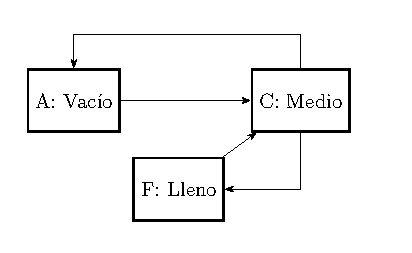
\includegraphics[width=0.7\textwidth]{ImagenesEjercicio1/Bloques-TT.pdf}
	\caption{Finite state machine.}
	\label{fig:fsm}
\end{figure}

Con lo presentado en la Figura (\ref{fig:fsm}), se confecciona una tabla de transiciones.
\begin{table}[H]
\centering
\begin{tabular}{|c|cccc|cc|}
\hline
\textbf{Estado Acutal} & \multicolumn{4}{c|}{\textbf{Estado Futuro}} & \multicolumn{2}{c|}{\textbf{Salida}} \\ \hline
                       & I-S       & I-S       & I-S      & I-S               & Both        & Toggle        \\
                       & 0-0       & 0-1       & 1-0      & 1-1                  &            &           \\ \hline
A                      & x         & x         & B        & x                   & 1          & 0         \\ \cline{1-1}
B                      & A         & x         & x        & C                  & 0          & 1         \\ \cline{1-1}
C                      & x         & x         & B        & x                  & 0        & 0  \\ \hline
\end{tabular}
\caption{Tabla de transiciones del sistema.}
\label{tab:estados}
\end{table}

A partir de la Tabla (\ref{tab:estados}) y la Figura (\ref{fig:fsm}) se puede llegar a la siguiente tabla, donde $y_1$ e $y_2$ representan la salida de los flip-flops, mientras que $Y_1$ e $Y_2$ la entrada de los mismos.
\begin{table}[H]
\centering
\begin{tabular}{|cc|cccc|cc|}
\hline
\textbf{Estado Acutal}  & \textbf{Codificación} & \multicolumn{4}{c}{\textbf{Estado Futuro}}                                                                                                                                                                                                                         & \multicolumn{2}{c|}{\textbf{Salida}} \\ \hline
\multicolumn{1}{|c|}{}  & $y_2 - y_1$           & \begin{tabular}[c]{@{}c@{}}$Y_2 - Y_1$\\ I-S\end{tabular} & \begin{tabular}[c]{@{}c@{}}$Y_2 - Y_1$\\ I-S\end{tabular} & \multicolumn{1}{c|}{\begin{tabular}[c]{@{}c@{}}$Y_2 - Y_1$\\ I-S\end{tabular}} & \begin{tabular}[c]{@{}c@{}}$Y_2 - Y_1$\\ I-S\end{tabular} & Ambos            & Toggle            \\
\multicolumn{1}{|c|}{}  &                       & 0-0                                                       & 0-1                                                       & \multicolumn{1}{c|}{1-0}                                                       & 1-1                                                       &                  &                   \\ \hline
\multicolumn{1}{|c|}{A} & 00                    & x                                                         & x                                                         & 01                                                                             & x                                                         & 1                & 0                 \\ \cline{1-1}
\multicolumn{1}{|c|}{B} & 01                    & 00                                                        & x                                                         & x                                                                              & 11                                                        & 0                & 1                 \\ \cline{1-1}
\multicolumn{1}{|c|}{C} & 10                    & x                                                         & x                                                         & 01                                                                             & x                                                         & 0                & 0                 \\ \cline{1-1}
\multicolumn{1}{|c|}{D} & 11                    & x                                                         & x                                                         & x                                                                              & x                                                         & x                & x                 \\ \hline
\end{tabular}
\end{table}

Se destaca que la variable ``Ambos'' hace referencia a estado en el cual se deben prender ambas bombas, mientras que la variable ``Toggle'' a cuando debe prenderse una sola e intercambiar.

Luego, se prosigue a resolver los mapas de Karnaugh para cada variable:

\begin{figure}[H]
\centering
\begin{subfigure}{.49\textwidth}
\centering
	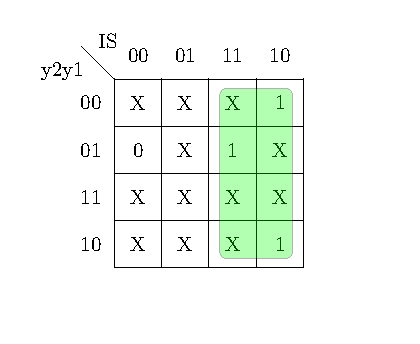
\includegraphics[width=0.7\textwidth]{ImagenesEjercicio1/Mapa1.pdf}
	\caption{Tabla de Karnaugh para $Y_1$.}
	\label{fig:fsm1}
\end{subfigure}
\begin{subfigure}{.49\textwidth}
\centering
	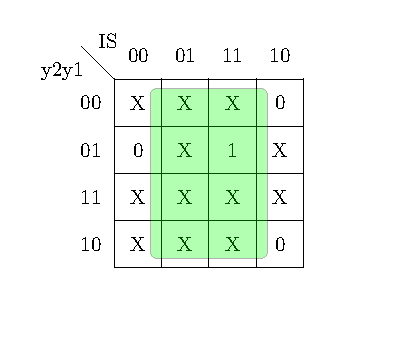
\includegraphics[width=0.7\textwidth]{ImagenesEjercicio1/Mapa2.pdf}
	\caption{Tabla de Karnaugh para $Y_2$.}
	\label{fig:fsm2}
\end{subfigure} \\
\begin{subfigure}{.49\textwidth}
\centering
	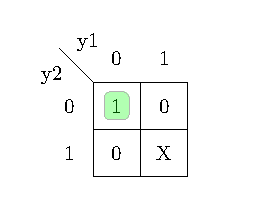
\includegraphics[width=0.5\textwidth]{ImagenesEjercicio1/Mapa3.pdf}
	\caption{Tabla de Karnaugh para ``Ambos''.}
	\label{fig:fsm3}
\end{subfigure}
\begin{subfigure}{.49\textwidth}
\centering
	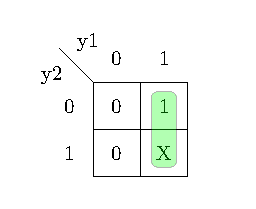
\includegraphics[width=0.5\textwidth]{ImagenesEjercicio1/Mapa4.pdf}
	\caption{Tabla de Karnaugh para ``Toggle''.}
	\label{fig:fsm4}
\end{subfigure}
\caption{Tablas de Karnaugh para cada variable analizada.}
\label{fig:kar}
\end{figure}

A partir de la Figura (\ref{fig:kar}) se derivan las siguientes expresiones:
\begin{equation}
\begin{split}
	Y_1 = & I \\
	Y_2 = & S 
\end{split}
\end{equation}
\begin{equation}
\begin{split}
Ambos = & \ \overline{y_2+y_1} \\
Toggle = & \ y_1
\end{split}
\end{equation}

Luego, se procede a obtener los circuitos para la FSM.
\begin{figure}[H]
\centering
	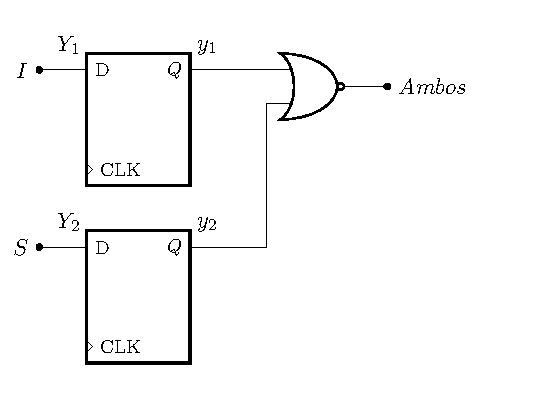
\includegraphics[width=0.6\textwidth, page=1]{ImagenesEjercicio1/Circuitos.pdf}
		\caption{Circuito FSM.}
	\label{fig:fsm1}
\end{figure}

Agregando el siguiente circuito lógico, se implementa la función de Toggle junto a la lógica de salida.
\begin{figure}[H]
	\centering
	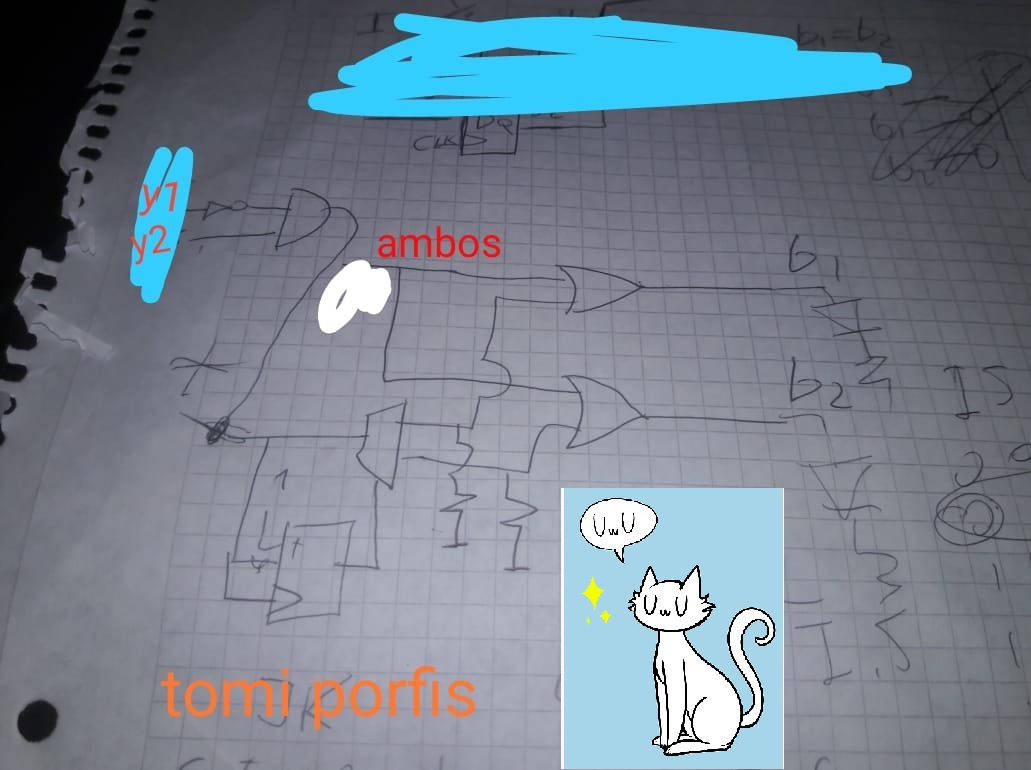
\includegraphics[width=0.7\textwidth]{ImagenesEjercicio1/post_logic.jpeg}
	\caption{Circuito FSM con Toggle.}
	\label{fig:fsm2}
\end{figure}
A partir de estos circuitos se realizó el PCB del mismo:
 \begin{figure}[H]
	\centering
	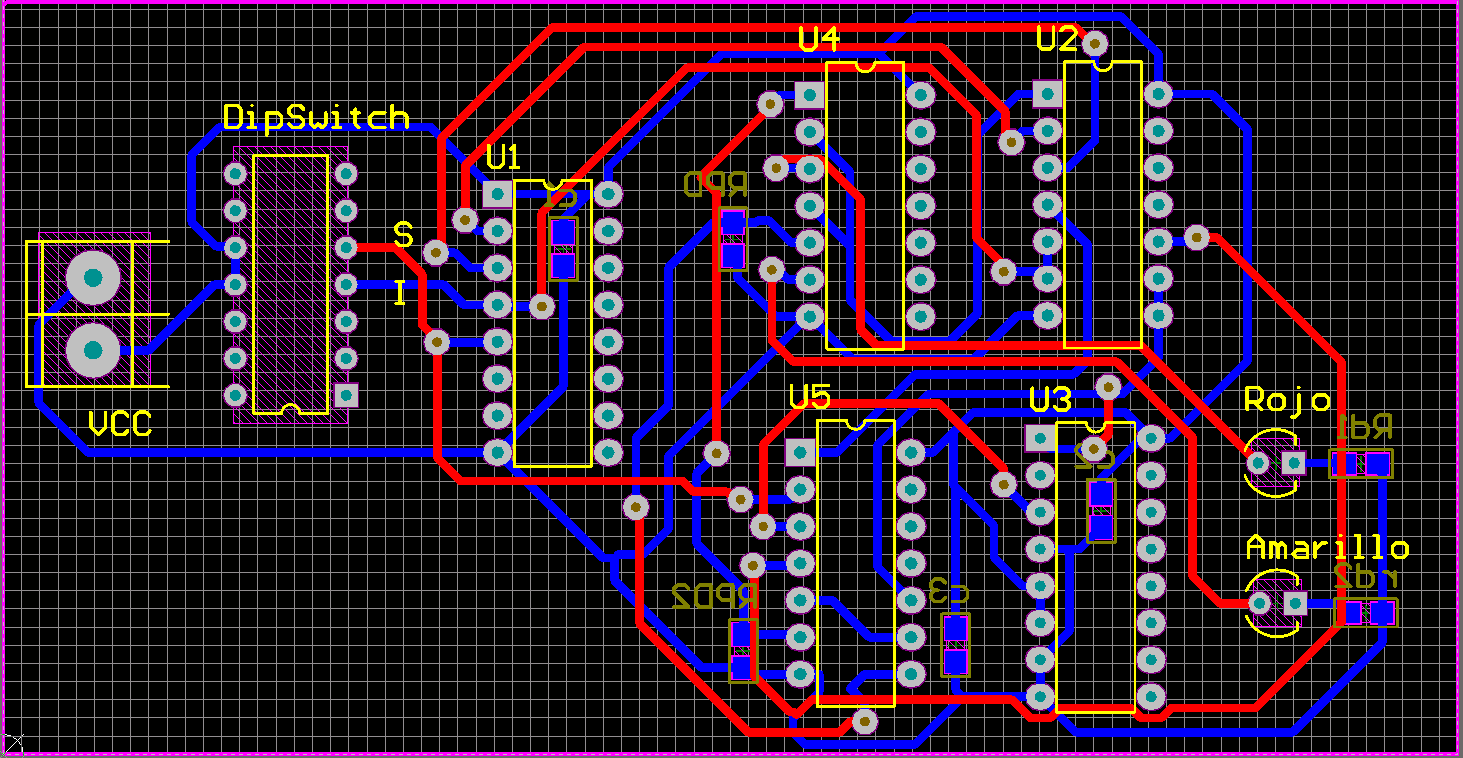
\includegraphics[width=0.7\textwidth]{ImagenesEjercicio1/PCB.PNG}
	\caption{PCB.}
	\label{fig:fsm}
\end{figure}
Dicha placa se llevo a cabo con resultados positivos.
 \begin{figure}[H]
	\centering
	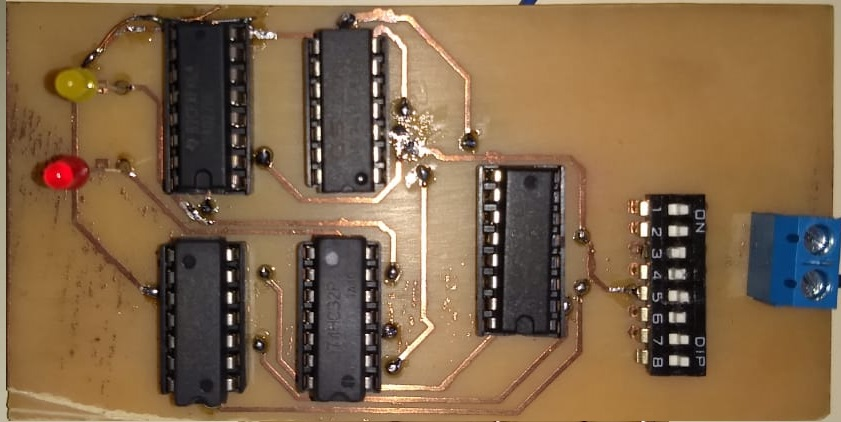
\includegraphics[width=0.8\textwidth]{ImagenesEjercicio1/pcbReal.jpeg}
	\caption{PCB implementado.}
	\label{fig:fsm}
\end{figure}
Luego se proecidió a medir los niveles de tensión para las transiciones posibles:
 \begin{figure}[H]
	\centering
	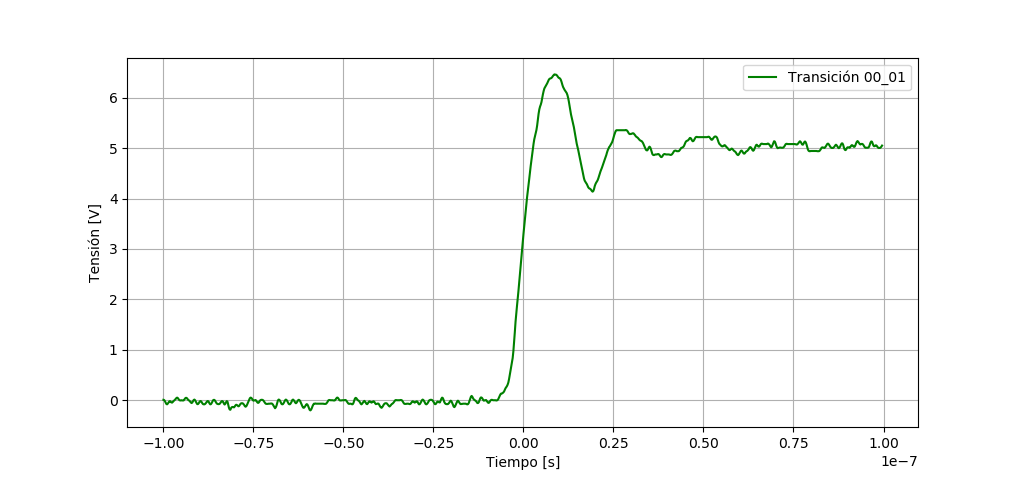
\includegraphics[width=0.8\textwidth]{ImagenesEjercicio1/00-01.PNG}
	\caption{Transición 00-01.}
	\label{fig:0001}
\end{figure}
 \begin{figure}[H]
	\centering
	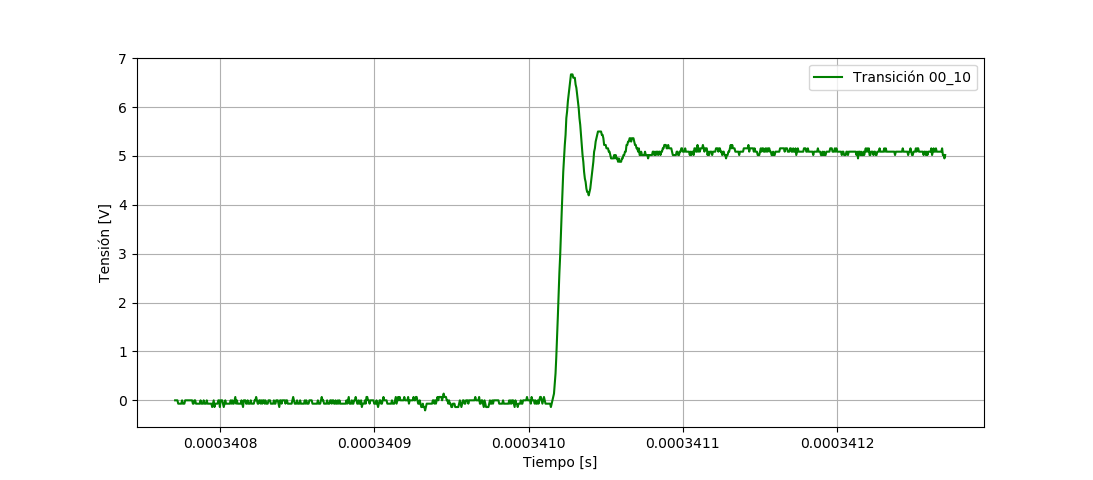
\includegraphics[width=0.8\textwidth]{ImagenesEjercicio1/00-10.PNG}
	\caption{Transición 00-10.}
	\label{fig:0010}
\end{figure}
 \begin{figure}[H]
	\centering
	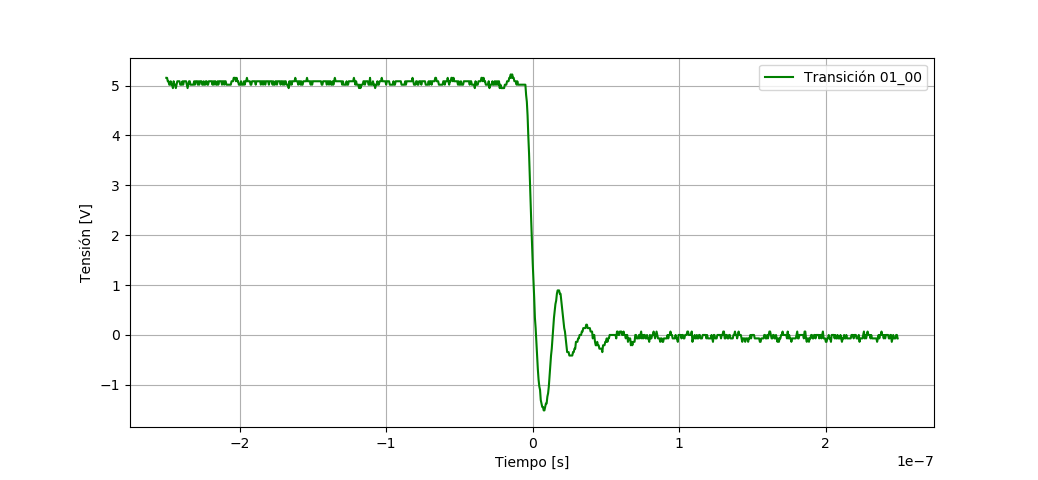
\includegraphics[width=0.8\textwidth]{ImagenesEjercicio1/01-00.PNG}
	\caption{Transición 01-00.}
	\label{fig:0100}
\end{figure}
 \begin{figure}[H]
	\centering
	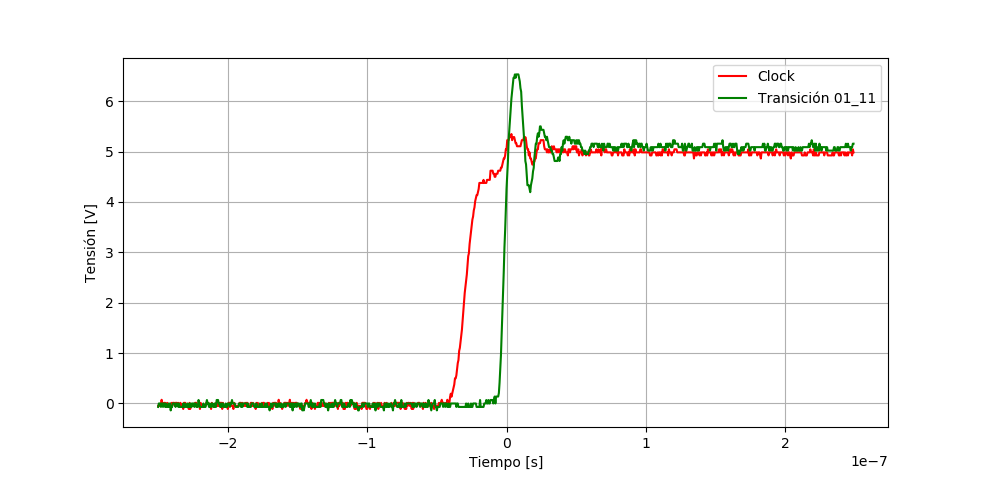
\includegraphics[width=0.8\textwidth]{ImagenesEjercicio1/01-11.PNG}
	\caption{Transición 01-11.}
	\label{fig:0111}
\end{figure}
 \begin{figure}[H]
	\centering
	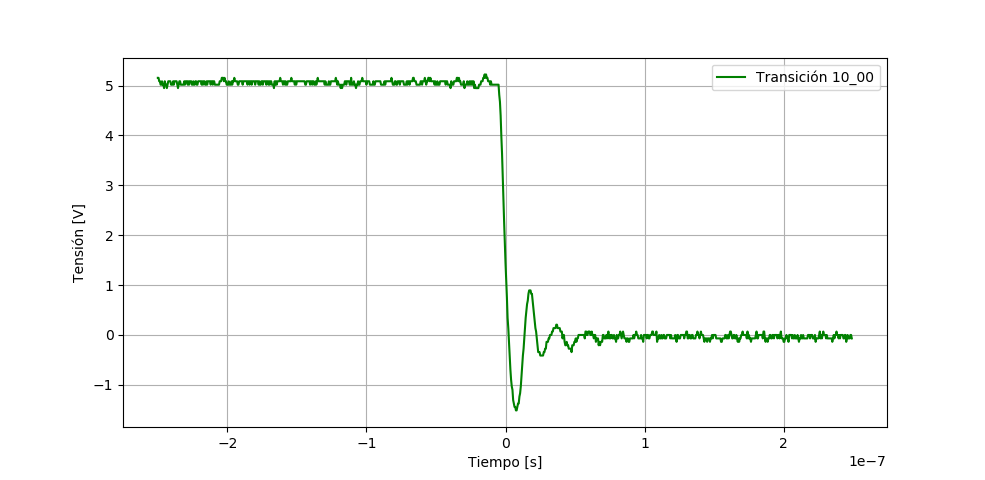
\includegraphics[width=0.8\textwidth]{ImagenesEjercicio1/10-00.PNG}
	\caption{Transición 10-00.}
	\label{fig:1000}
\end{figure}
 \begin{figure}[H]
	\centering
	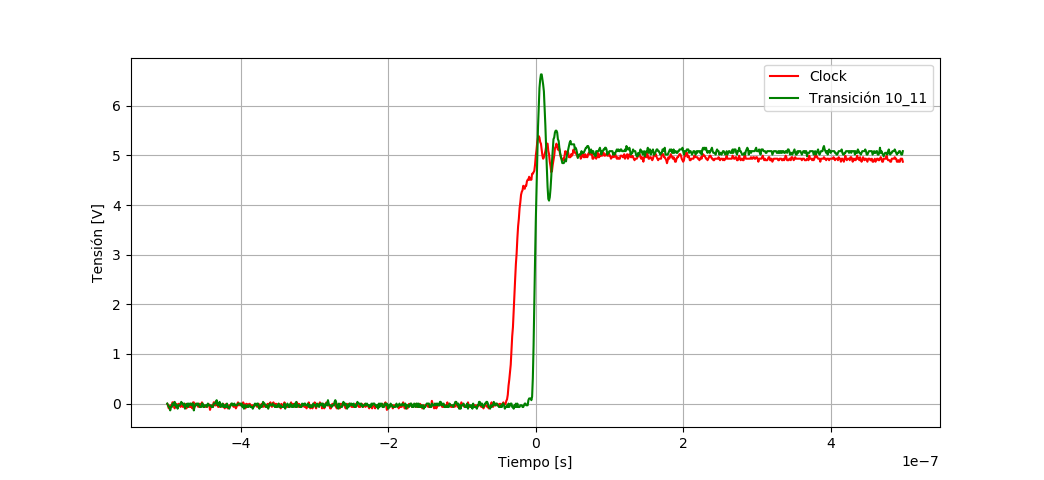
\includegraphics[width=0.8\textwidth]{ImagenesEjercicio1/10-11.PNG}
	\caption{Transición 10-11.}
	\label{fig:1011}
\end{figure}
 \begin{figure}[H]
	\centering
	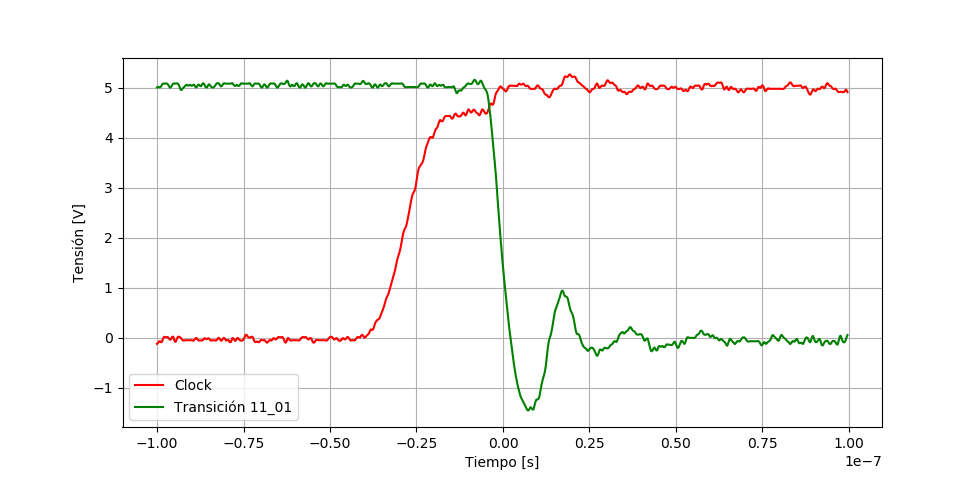
\includegraphics[width=0.8\textwidth]{ImagenesEjercicio1/11-01.PNG}
	\caption{Transición 11-01.}
	\label{fig:1101}
\end{figure}
 \begin{figure}[H]
	\centering
	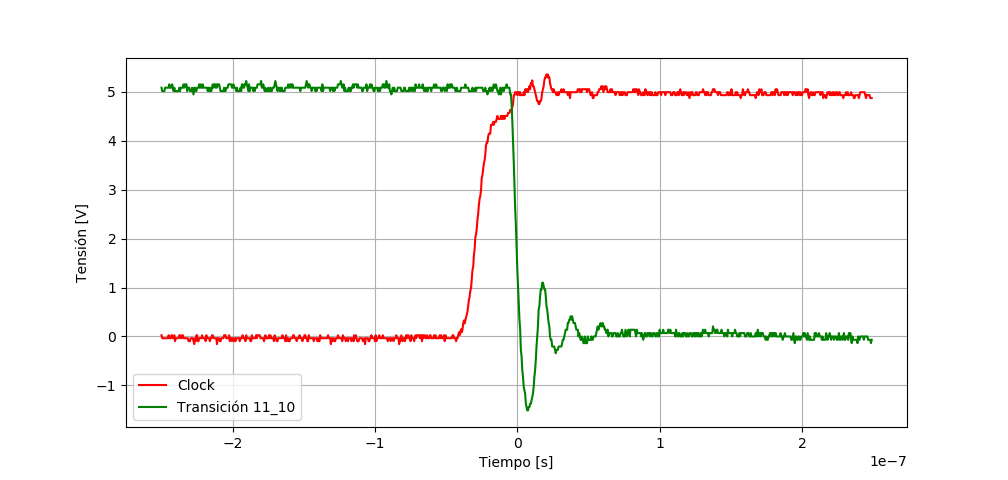
\includegraphics[width=0.8\textwidth]{ImagenesEjercicio1/11-10.PNG}
	\caption{Transición 11-10.}
	\label{fig:1110}
\end{figure}
\end{document}